\documentclass{beamer}

\usepackage[utf8]{inputenc}
\usepackage{default}
\usepackage{caption}
\begin{document}
\begin{frame}{Dependency Path Based Relation Extraction}{Peculiarity of Numerical Relations}
\begin{itemize}
 \item Analyzing a number of sentences expressing numerical relations lead to several insights as already discussed. \\
 \item \textbf{Keywords} We can expect presence of certain keywords that might help in identifying relations.\\
 \item \textbf{Modifiers} A large number of false positives stem out of mentions where a change in the numerical attribute is mentioned.
\end{itemize}
\end{frame}

\begin{frame}{Dependency Path Based Relation Extraction}{Dependencies}
\begin{itemize}
 \item Dependencies: Grammatical relation between two words, governer and dependent. \\
 \item ``The red ball was lost'' \\
\item \begin{itemize}
\item \textbf{amod(ball,3,red,2)} ``Red'' is an adjective for ``ball''
\item \textbf{det(ball,3,The,1)}  ``the'' is a determiner of ``ball''
\item \textbf{nsubjpass(lost,5,ball,3)}	``ball is the subject of lost''
\item \textbf{auxpass(lost,5,was,4)}	``was is an auxiliary of lost''
\end {itemize}
\end{itemize}
\begin{figure}[h]
 \centering
 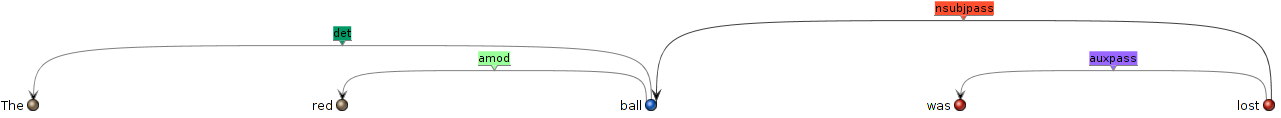
\includegraphics[bb=0 0 1281 118,scale=0.25]{./imgs/dep.png}
 % dep.png: 1281x118 pixel, 72dpi, 45.19x4.16 cm, bb=0 0 1281 118
\end{figure}

\end{frame}

\begin{frame}{Dependency Path Based Relation Extraction}
 
\begin{itemize}
 \item Given a Country-Number pair, extract the shortest undirected path between them in the dependency graph.
\end{itemize}
 \begin{figure}[h]
 \centering
 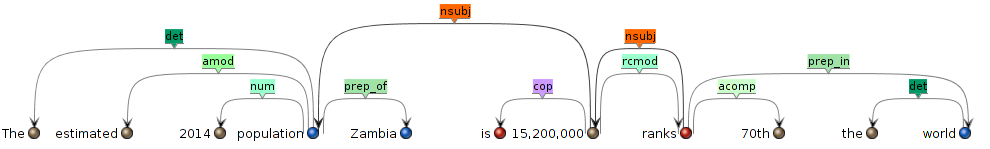
\includegraphics[bb=0 0 990 149,scale=0.3]{./dep.png}
 % dep.png: 990x149 pixel, 72dpi, 34.92x5.26 cm, bb=0 0 990 149
\end{figure}
\begin{itemize}
 \item Path(Zambia - 15,200,000) = \{Zambia, population, 15,200,000\}
  \item For a match, the path:
  \begin{itemize}
   \item Should have one of the keywords
   \item Should not have a modifier
  \end{itemize}
 \end{itemize}
\end{frame}

\begin{frame}{Dependency Path Based Relation Extraction}{Example}
\begin{figure}[h]
 \centering
 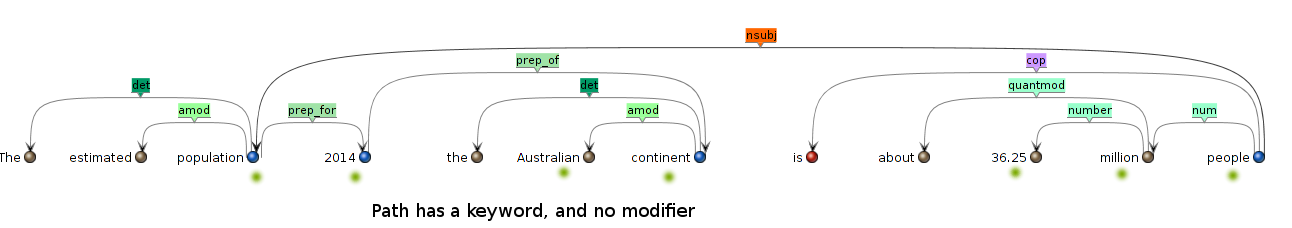
\includegraphics[bb=0 0 1292 228,scale=0.25]{./dep_pos.png}
 % dep_pos.png: 1292x228 pixel, 72dpi, 45.57x8.04 cm, bb=0 0 1292 228
 \caption*{Extracted}
\end{figure}
\begin{figure}[h]
 \centering
 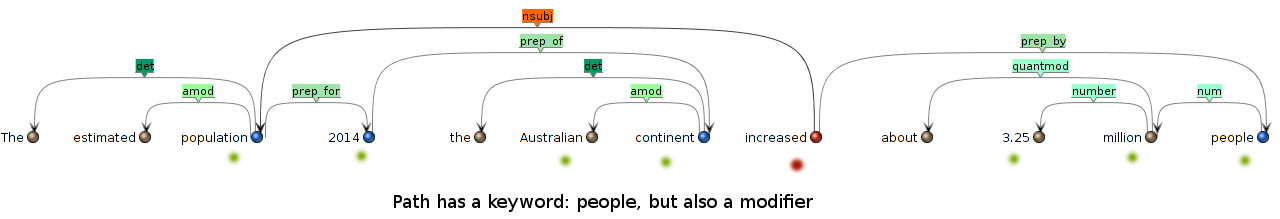
\includegraphics[bb=0 0 1280 219,scale=0.25]{./dep_neg.png}
 % dep_neg.png: 1280x219 pixel, 72dpi, 45.15x7.72 cm, bb=0 0 1280 219
 \caption*{Not Extracted}
\end{figure}

\end{frame}

\begin{frame}
\begin{itemize}
\item The extractor was applied to 30 sentences expressing 23 different relations. \\

\item \resizebox{\linewidth}{!}{% Resize table to fit within \linewidth horizontally
 
\begin{tabular}{|l|l|l|}
\hline
& Relations Present & Relations not Present (False positives) \\
\hline
Extracted & 16 & 17 \\
\hline
Not Extracted & 7 & N/A \\
\hline
\end{tabular}}

 \begin{itemize}
  \item Precision: 48.4\%
  \item Recall: 69.6\%
 \end{itemize}

\item The precision will increase further on applying unit based pruning.	
\end{itemize}

\end{frame}

\end{document}
